\documentclass[]{article}

\usepackage{graphicx}
\usepackage{amsmath}
\usepackage{amsfonts}
\usepackage{amssymb}
\usepackage[left=3cm, right=3cm]{geometry}

%opening
\title{Conceptual Framework for Learning and Cognition}
\author{Diego Bonilla Salvador\\
\texttt{diegobonila@gmail.com}}

\begin{document}

\maketitle

\begin{abstract}
We present a formal framework for modeling learning and understanding in systems. This framework is a high-level, abstract model of how an entity (biological or artificial) transforms sensory inputs into meaningful outputs through internal functions. With the use of consistent notation and systematical organization of the ideas, we hope this can serve as a reference model for modeling such interaction between systems. This framework is a formal restatement and synthesis of existing concepts, unifying concepts from different fields such as systems theory, learning processes, neural networks and evolutionary biology. The whole framework is grounded in set theory, functional analysis, and decision theory.
\end{abstract}

\section{Introduction}
This article provides a unified, formal framework for understanding how systems acquire, interpret, and act upon information. It highlights that any system’s knowledge and understanding arise from its internal mapping of sensory inputs to outputs, shaped by value and cost functions, and constrained by its architecture. We assume that each system only observes the world through its own sensory channels, that its capacity for conceptualizing and responding to the environment is limited and can change over time, and that learning is guided by intrinsic and extrinsic signals. Under these assumptions, intelligence, understanding, and communication between different minds are shown to depend on overlapping representational capabilities and the interplay between internal conceptual structures and external feedback.

\section{Basic Elements}

We outline the basic elements and formalizations that introduce this framework.

\begin{figure}[h]
	\centering
	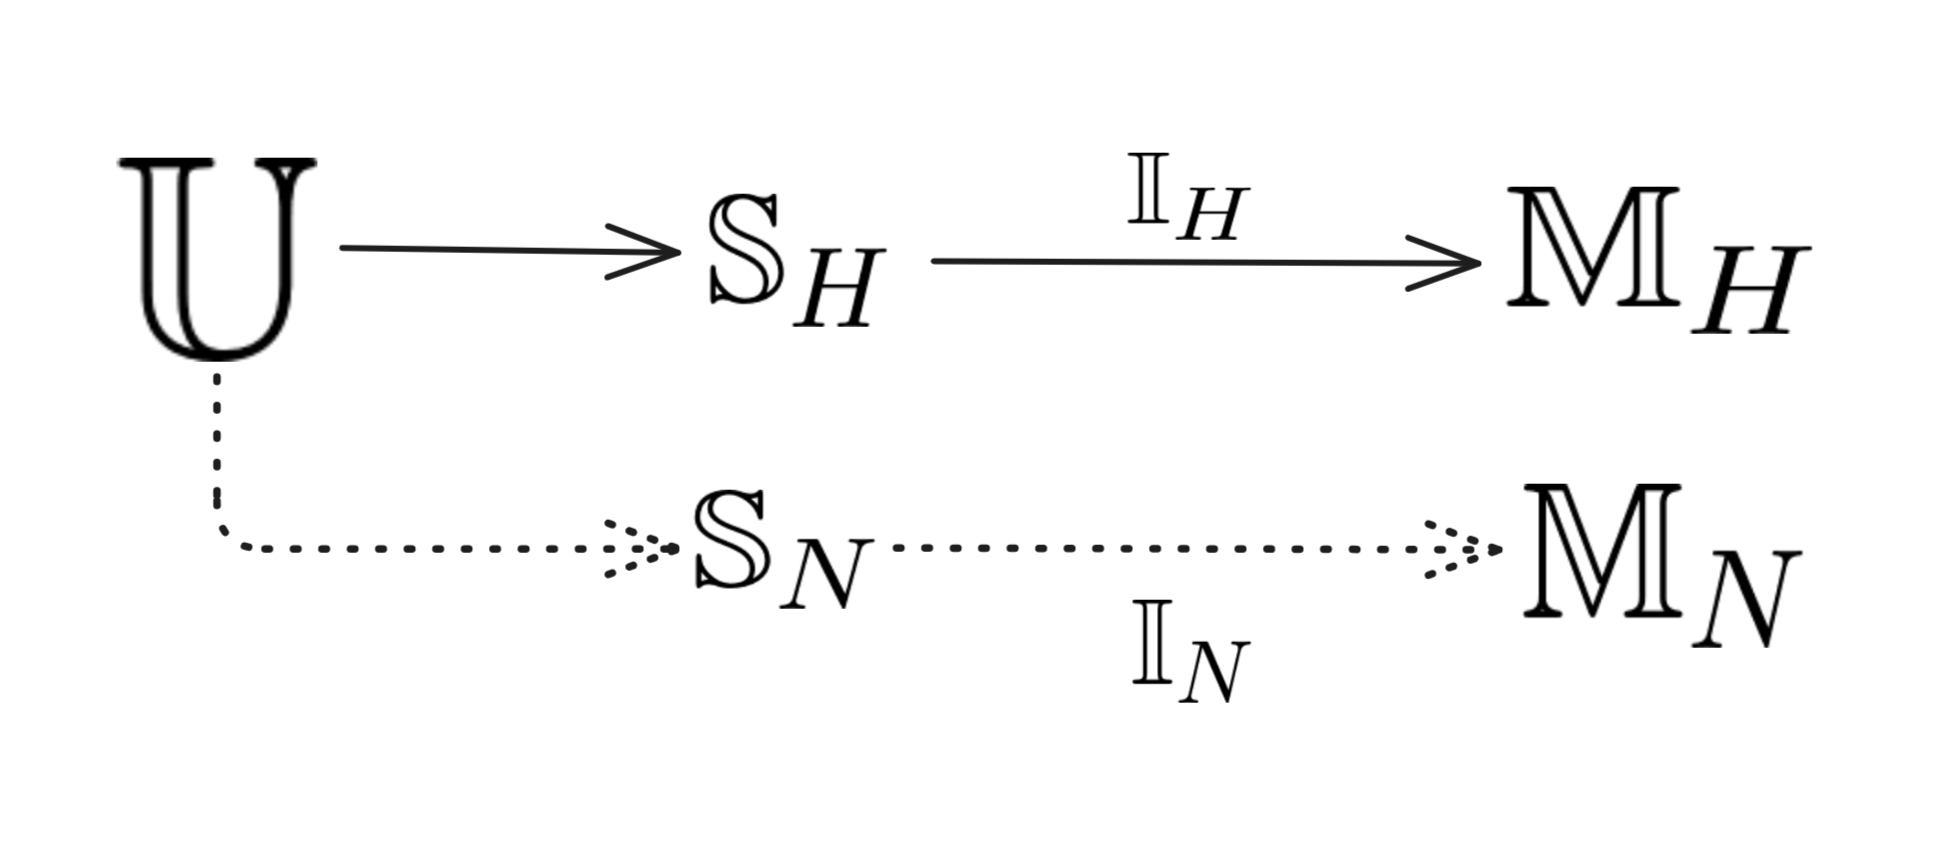
\includegraphics[width=0.5\textwidth]{basic}
	\caption{Basic outline of the framework. A system $\mathbb{B}_H$ receives sensory data $s_H \in \mathbb{S}_H$ from the universe $\mathbb{U}$. The system converts the input sensory data into physical outputs $m_H \in \mathbb{M}_H$. Another system has different processes but same universe to receive inputs from.}
	\label{fig:fig1}
\end{figure}

\subsection{Environment and Perception}
\begin{itemize}
	\item \textbf{Universe} ($\mathbf{U}$): Let $U$ be a set representing all possible states of the environment external to the system.
	\item \textbf{Sensing and Input Space} ($\mathbf{S}$): The system does not directly observe $U$. Instead, it has a sensing function:
	\[ \phi: U \to S \]
	where $S$ is the set of all possible sensory inputs the system can receive. For any $u \in U$, the system perceives $s = \phi(u) \in S$. We suppose this mapping is surjective since no system can be as complex as the universe around it. Critically, the system’s knowledge of $U$ is always mediated by $\phi$.
\end{itemize}

\subsection{Action and Output Space}
\begin{itemize}
	\item \textbf{Output or Action Space} ($\mathbf{M}$): The system responds to inputs $s \in S$ by producing physical outputs $m \in M$. These output may in turn affect $U$, closing the loop:
	\[ U \xrightarrow{\phi} S \xrightarrow{f} M \xrightarrow{\psi} U', \]
	where $\psi$ represents how outputs act back on the environment, possibly changing its state to $U'$. Neither $\phi$ nor $\psi$ are necessarily known or invertible from the system's perspective.
\end{itemize}

\subsection{Function Space and Representational Constraints}
\begin{itemize}
	\item \textbf{Set of All Possible Functions} ($\mathbf{I}$): Consider all functions $f: S \to M$. The collection of these functions is:
	\[ I = \{ f \mid f: S \to M \}. \]
	We suppose possible physical systems have finite $S$ and $M$ sets. Thus, $| I | = | M | ^ {| S |}$ defines the theoretical space of all behaviors, though the system may realize only a subset due to internal structure.
	\item \textbf{Feasible Function Space} ($\mathbf{E}$): $|I|$ can be enormous, no system can explore all functions. Its architecture limits can be represented and learned in $E$. Let $E \subset I$ be the subset of function that the system can execute with its current internal architecture. Changes in the system internal mappings (in humans can mean synaptogenesis or in neural networks changing the architecture) can expand $E$, while, for example, damage can reduce it.
\end{itemize}

\subsection{Value and Cost Functions}
We define two hypothetical functions that measure how good an output is.
\begin{itemize}
	\item \textbf{Value Function} ($\mathbf{V}$):
	\[ V: S \times M \to \mathbb{R}, \]
	Internal function that assigns a real number to each input-output pair $(s, m)$. For a fixed $s$, $V(s, m)$ indicates the immediate desirability or utility of choosing $m$ in response to $s$.
	At any given moment, the system chooses:
	\[ f(s) = \arg \max_{m \in M} V(s, m) \]
	Thus, $V$ directly determines the system's policy for action selection, given its current internal model. This is the immediate "policy-level" function guiding behavior.
	\item \textbf{Cost Function} ($\mathbf{V}$): The cost function, $C$, provides a meta-level shaping criterion that influences how $V$ is adapted over time.
	\[ C: S \times M \to \mathbb{R}, \]
	The cost function is an external signal that models a system's behavior.
\end{itemize}
In other words, $V$ determines which action is chosen at a given time; $C$ determines how $V$ changes over time, indicating how learning should proceed to better align the system's behavior with given goals. Every system contains a pre-defined $V$ based on the nature of the system itself, we can call this \textbf{inductive bias}. Is the definition of $C$ that models the concepts of \textit{understanding} and \textit{learning} in a system.

\section{Conceptual Structures and Understanding}
We mentioned that \textit{understanding} is given by the criteria $C$. Without this criteria, there is no distinction between meaningful outputs and random noise. For example, a neural network trained to classify cats and dogs can take as input the image of a car, but we, as humans, will interpret the output as random noise (or as having none information), this is because we set the criteria $C$ during training that network and during the evaluation. The network's $V$ function will still output the best action possible even if it does not align with $C$.
In this section, we suppose a condition $C$ is given and we can differentiate between what a system can \textit{process} and what it can \textit{understand}. We use sigma-algebra to make this distinction.
\begin{itemize}
	\item \textbf{Conceptual Sigma-Algebra} ($\mathcal{F}$): Let $(S, \mathcal{F})$ be a measurable space where $\mathcal{F}$ is a sigma-algebra on $S$. Elements of $\mathcal{F}$ are sets of inputs that the system can conceptualize or partition meaningfully. We interpret each $A \in \mathcal{F}$ as a "conceptual category" the system can internally represent.
	\item \textbf{Understanding and Interpretation}: The system "understands" a subset $A \subseteq S$ if it can:
	\begin{enumerate}
		\item Recognize $A$ as a meaningful category (i.e., $A \in \mathcal{F}$).
		\item Produce outputs $f(s)$ for $s \in A$ that align with external criteria $C$ (e.g., consistently high values as judged by the value function $V$).
	\end{enumerate}
\end{itemize}
As we mentioned, \textit{understanding} is an actor-dependent term: different systems have different $\mathcal{F}$ and different alignment criteria $C$. The concept of "learning" can be easily defined as understanding some given $s \in S$ and a $C$ over time such that $\mathcal{F}_t \subset \mathcal{F}_{t+1} \subset \mathcal{F}_{t+2} \cdots$ and similarly expanding $E$.

The difference between $E$ and $\mathcal{F}$ is that $E$ relates to the space of behaviors the system can exhibit, while $\mathcal{F}$ relates to the space of conceptual distinctions the system can internally represent.


\section{Inter-System Communication and Imitation}
Consider two systems, $System_1$ and $System_2$. Each has its how set of possible inputs $S$, mapping functions $I$, and possible outputs $M$. It is possible for $System_1$ to map $System_2$ mapping functions back to its own, essentially "understanding" the thought process of the other system. We refer to this process as process $\mathbf{B}$.\\
Since the $System_2$ outputs $m_2$ modify the universe $U$, $System_1$ can directly sense the result $s_1$ and attempt to reverse mapping $B$ to approximate $f_2$ from within its own representational constraints. However, this interpretability is limited. If the manifolds of representable functions $I_1$ and $I_2$ do not overlap, or if $\mathcal{F}_1$ and $\mathcal{F}_2$ carve up $S$-spaces differently, true understanding might fail.

\begin{figure}[h]
	\centering
	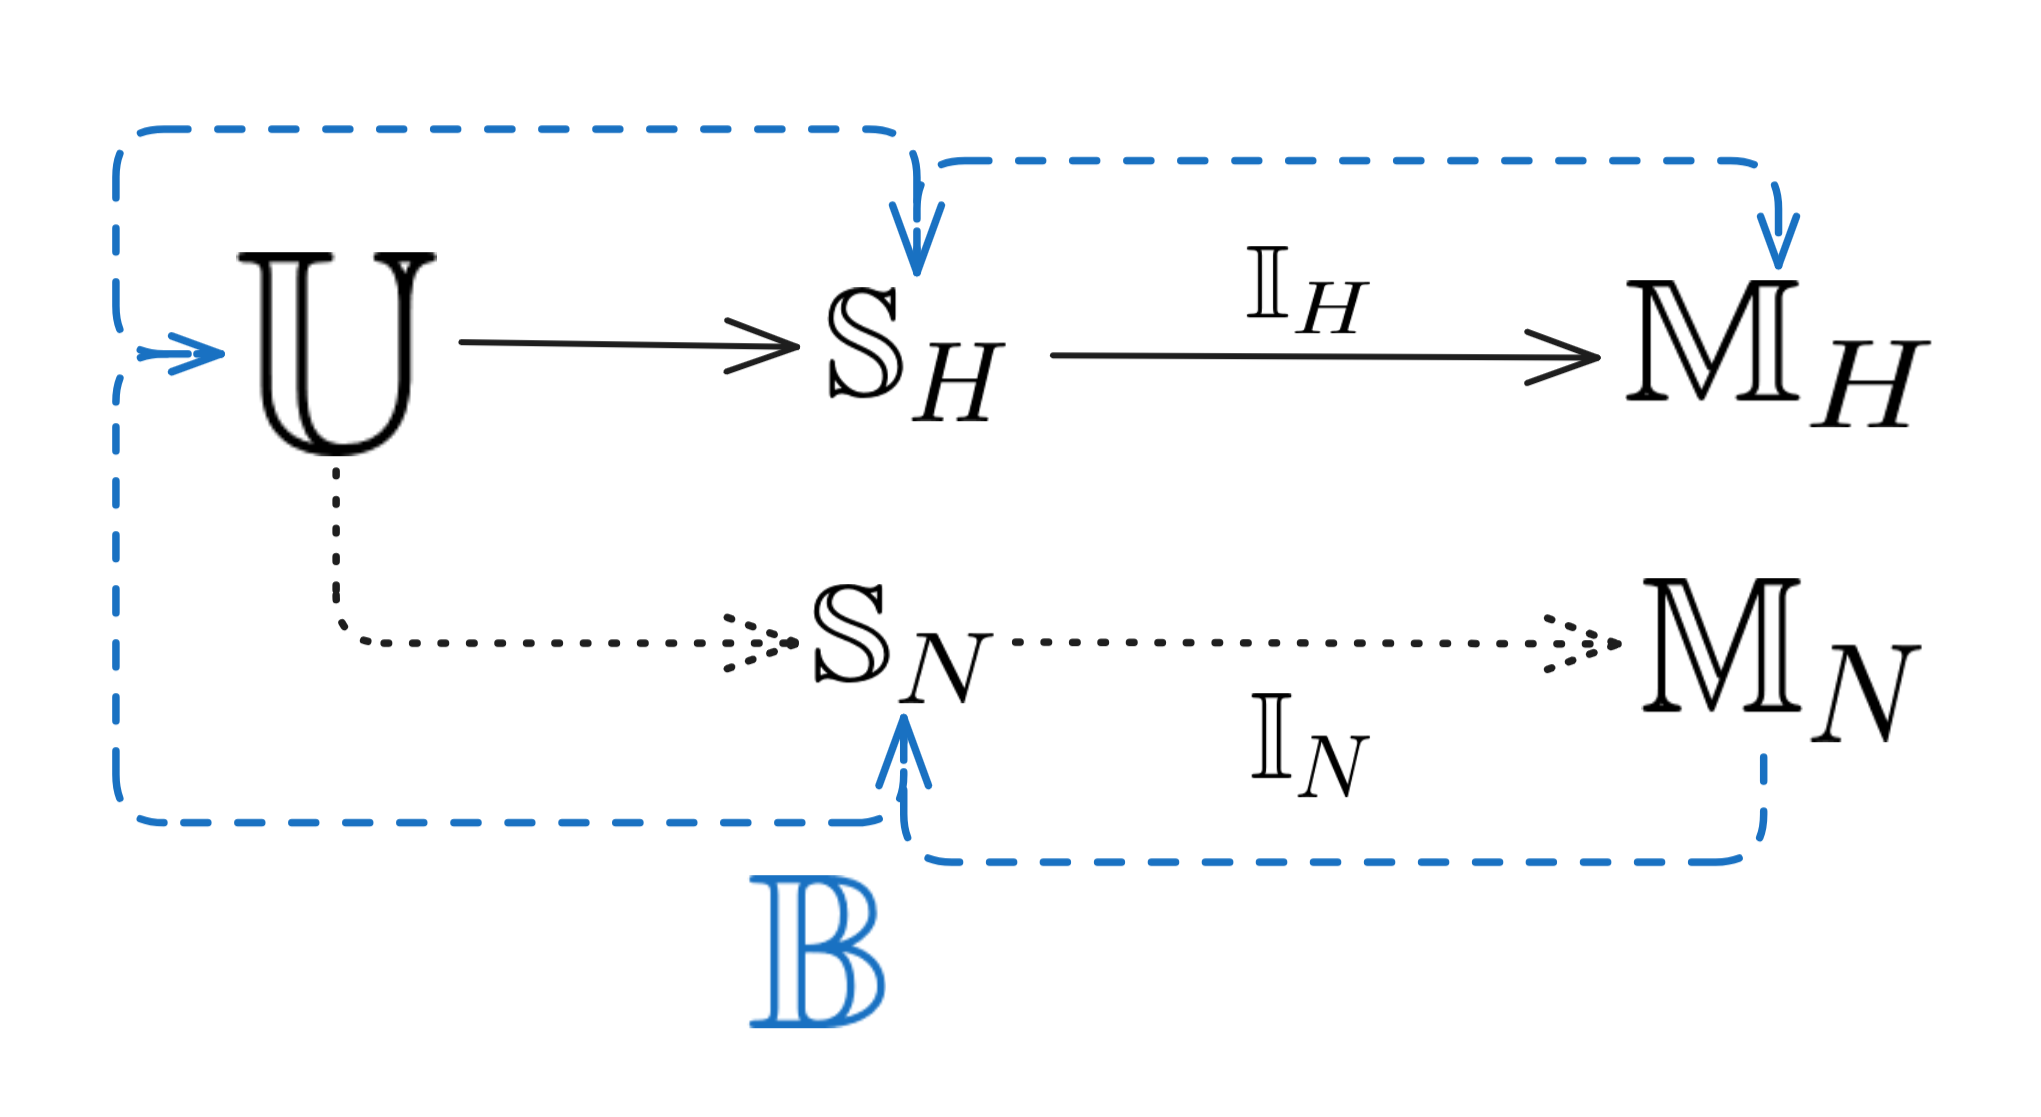
\includegraphics[width=0.5\textwidth]{b}
	\caption{Basic outline of the process $B$. System $H$ can partially understand system $N$.}
	\label{fig:fig2}
\end{figure}

We can define there exists subsets $J_1$ of $I_1$ and $J_2$ of $I_2$ of the same size, and that applying the process $B$ to $J_1$ yields exactly $J_2$.
\[
\exists J_1 \subseteq I_1,\; \exists J_2 \subseteq I_2 : \quad |J_1| = |J_2| \;\wedge\; B(J_1) = J_2.
\]
In other words, a subset of one set can be transformed into a subset of the other via process $B$.

Formulated differently, we can restrict the subset of $I_1$ to only come from the intersection information of $I_1$ and $B(I_N)$:
\[
\exists J_2 \subseteq I_2 : \exists J_1 \subseteq (I_1 \cap B(I_2)) \quad \text{such that} \quad |J_1| = |J_2| \;\wedge\; B(J_1) = J_2.
\]
This ensures that we only consider those elements in $I_1$ that can be obtained by applying $B$ to some elements of $I_1$.

Furthermore, if imitation is possible, $System_1$ uses $C$ to modify its $V$, aligning its behavior closer to the perceived strategy of $System_2$, thereby "learning by imitation". This is how neural networks learn and how different species are able to communicate.

The "intellectual proximity" can be defined as $|J_\bullet|$ and defines the possibility of practical communication between these two systems.

\subsection{Ensemble of Systems}
For this section, we assume constant shared $C$ and that systems can "communicate" to each other.
\begin{itemize}
	\item Suppose the ensemble $\{ \mathbb{B}_\alpha \}$ can communicate and share representational structures. We might consider the formation of a collective feasible set of functions. The intuitive idea is that if systems can share representations, they can potentially "learn" from each other and possibly realize a larger set of functions collectively than any individual system alone.
	\item We define a collective feasible set $E^{\text{coll}}$ as follows. Let:
	\[ E^{\text{coll}} \subset \prod_{\alpha \in A}^{} I_\alpha \]
	represent sets of tuples of functions $(f_\alpha)_{\alpha \in A}$ where each $f_\alpha \in E_\alpha$. This is a direct product space of each system’s feasible sets. However, simply forming a product of each system’s feasible set does not automatically increase any individual system’s own feasible set. They remain structurally limited individually.
	
	To allow for interaction, consider that systems attempt a form of "alignment" via the process $B$. If system $\alpha$ can interpret subsets of $I_\beta$ under $B_{\alpha,\beta}$, it might be able to adjust its architecture to incorporate patterns from $\beta$. Over time, one might define an interactive procedure where:
	\begin{enumerate}
		\item Each system $\mathbb{B}_\alpha$ attempts to enlarge its feasible set $E_\alpha$ by including functions that it can approximate from the image under $B_{\alpha,\beta}$ for some $\beta$.
		\item Similarly, each system tries to refine its conceptual $\sigma$-algebra $\mathcal{F}_\alpha$ by including sets it can now differentiate due to newly acquired representational abilities.
	\end{enumerate}
	
	\item The intellectual proximity $|J|$ plays a big factor. If $|J|$ is large, that means a significant portion of one system’s representable functions can be translated into another system’s language of functions. This large overlap allows the systems to "communicate" effectively about complex behaviors and possibly share conceptual structures.
	
	\item Consider an iterative operator $\mathcal{T}$ acting on the family $\{( E_\alpha, \mathcal{F}_\alpha )\}_{\alpha \in A}$:
	\[  \mathcal{T} \Big( \{( E_\alpha, \mathcal{F}_\alpha )\}_{\alpha \in A} \Big) = \{( E'_\alpha, \mathcal{F}'_\alpha )\}_{\alpha \in A}. \]
	If $|J_{\alpha,\beta}|$ (the size of a matched pair under $B_{\alpha,\beta}$) is large for multiple pairs of systems $\alpha, \beta$, the iterative operator $\mathcal{T}$ may produce expansions in some $\mathcal{F}_\alpha$ and $E_\alpha$. Conversely, if $|J_{\alpha,\beta}|$ is small or zero, the exchange does not yield new representational patterns that are meaningful to the receiving system. Hence, no significant growth occurs.
\end{itemize}

However, this collaboration can also arise some problems:
\begin{itemize}
	\item \textbf{High Similarity Case}: Is all systems are very similar, say they have identical $(S_\alpha, M_\alpha)$ and initial $E_\alpha, \mathcal{F}_\alpha$, and high $|J_{\alpha, \beta}|$ for all pairs, then each is basically a mirror og the others. In this case, communication does not add fundamentally new distinctions. They might collectively stabilize at the same level of understanding as a single system. Hence, $\mathcal{F}^{\text{coll}}$ would not be significantly larger than $\mathcal{F}_\alpha$ for any $\alpha$.
	\item \textbf{High Diversity with Good Communication}: Suppose the systems differ initially (different $S_\alpha, M_\alpha, I_\alpha$) and yet large portions of their representational spaces can be mapped through $B$. This scenario allows for the greatest expansion. Over iterations, each system can incorporate new subsets into its conceptual structure. Collectively, $\mathcal{F}^\text{coll}$ is strictly larger than any single initial $\mathcal{F}_\alpha$.
	\item \textbf{High Diversity with Poor Communication}: If the system are very different, with negligible $|J_{\alpha,\beta}|$, then the process $B$ fails to map meaningful subsets of one system's representational set ot another. No significant transfer occurs. Each $\mathcal{F}_\alpha$ and $E_\alpha$ remains essentially the same. The collective does not approach a broader conceptual space.
\end{itemize}


\section{Implications}
Using this framework as reference, we can extract formalizations of several ideas from different fields, showing the capabilities of this framework to provide a unified, clear and formal definition for multiple disciplines.
\begin{itemize}
	\item The implication that $E \subset I$ simply states that the system's actual representable behaviors (the functions it can realize) form a proper subset of the space of all possible functions. It follows from the statement that the system is constrained by its architecture. If the system had no constraints, it could realize any function and would have $E = I$. In this article, we assume such system is not physically possible. In other words: a system cannot learn or understand everything.
	\item The system's conceptualization $(S, \mathcal{F})$ and the value structure $(C, V)$ define what it can "understand". Signals outside $\mathcal{F}$ remain incomprehensible or appear as noise. Another system might find them meaningful. We note then that the distinction between "noise" and "knowledge" is observer-relative, depending on internal constraints.
	\item Biological and computational constraints limit $I$ and the feasible subset $E$. Not all concepts in $\mathcal{F}$ can be understood simultaneously, and not all signals from $S$ can be interpreted meaningfully. Thus, there is an inherent limit to what a system can learn or understand, influenced by its architecture, evolutionary biases, internal value/cost functions, and the complexity of $U$.
	\item Intelligence or understanding are not absolute metrics. They depend on $C$ (the shaping forces), $V$ (the decision-making evaluation), and $\mathcal{F}$ (the conceptual partitions). Without these references, one cannot universally label a function $f$ as "intelligent" or "understanding."
	\item The process $B$ og interpreting another system's function set $I_2$ from the perspective of $I_1$ is fundamentally limited by representational intersections of $\mathcal{F}_1$ and $\mathcal{F}_2$. This yields a theoretical lower bound on inter-system communication: no matter how much data or imitation is attempted, if the conceptual manifolds do not share overlapping $\sigma$-algebraic structures, perfect mutual understanding is unattainable.
	\item The interplay between $C$ and $V$ creates a scenario where the system may settle into locally optimal conceptual frameworks. Because $C$ influences how $V$ changes, certain conceptual subsets in $\mathcal{F}$ become reinforced over time, pushing the system toward particular regions of $E$. This implies that learning trajectories are path-dependent: two systems with identical initial conditions but slightly different early perturbations to $V$ or $C$ may end up with radically different stable sets of conceptual categories and values. Thus, "cognitive attractors" emerge, where the system’s evolution in conceptual and behavioral space is not just about incremental improvement, but about becoming "trapped" in particular representational niches.
	\item Since sets not in $\mathcal{F}$ are uninterpretable data for the system, the framework implies a novel view of noise: it is not a property of the environment $U$ alone, but of the interaction between $U$ and $\phi$, relative to $\mathcal{F}$. This implies that trough learning with the correct $C$, a system can transform noise into knowledge without any external change in $U$. This, in this framework, noise is not a fixed attribute but rather a function of conceptual sophistication.
	\item The formal distinction between $C$ and $V$ and their influence on $\mathcal{F}$ and $E$ leads to the implication that two systems may not only disagree on what to do (due to different $V$) but may also be incapable of agreeing on how to improve (due to different $C$). This lack of a common improvement protocol means that even if two agents share a portion of conceptual space, their meta-level learning rules might prevent them from ever converging. Differences in $C$ produce non-reconcilable strategies for updating $V$.
	\item The existence of a universal $\mathcal{F}^*$ that captures all distinguishable subsets of $S$ would be too large to represent within any finite system's $E$. Thus, universal conceptual coverage is unattainable, and this limitation is fundamental, not merely practical. It follows that "complete understanding" of all sensory possibilities is not just unfeasible but mathematically out of reach given finite constraints on representational capacity given in this framework. This suggests that the universe, as approached by any finite intelligence, inherently contains horizons that cannot be crossed.
\end{itemize}

\end{document}









